%%%%%% CMB-S4 Neutrinos Chapter  %%%%%%%%%%%%%%%%
 
\chapter{Light Relics}
%\renewcommand*\thesection{\arabic{section}}


\def\beq{\begin{equation}}
\def\eeq{\end{equation}}

\def\bea{\begin{eqnarray}}
\def\eea{\end{eqnarray}}

\def\Neff{N_{\rm eff}}
\def\Nf{N_{\rm eff}}
\def\gs{g_{\star}}
\def\Mpl{M_{\rm pl}}
%\newcommand{\nucl}[3]{ \ensuremath{ \phantom{\ensuremath{^{#1}_{#2}}} \llap{\ensuremath{^{#1}}} \llap{\ensuremath{_{\rule{0pt}{.75em}#2}}} \mbox{#3} } }


\def\gtrsim{\raise-.75ex\hbox{$\buildrel>\over\sim$}}
\def\lsim{\raise-.75ex\hbox{$\buildrel<\over\sim$}}
%%%%%%%%%%%%%%%%%%%%%%%%%%%%%%%%%%%%%%%%%%%%%%%%%%%%%%%%%%%
%%%%%%%%%%%%%%%%%%%%%%%%%%%%%%%%%%%%%%%%%%%%%%%%%%%%%%%%%%%
%%%%%%%%%%%%%%%%%%%%%%%%%%%%%%%%%%%%%%%%%%%%%%%%%%%%%%%%%%%
%%%%%%%%%%%%%%%%%%%%%%%%%%%%%%%%%%%%%%%%%%%%%%%%%%%%%%%%%%%

\begin{center}
{\small \it (send feedback on this chapter to \href{mailto:s4_neutrinos@cosmo.uchicago.edu}{s4\_neutrinos@cosmo.uchicago.edu})}
\end{center}

\begin{quotation}

New light particles appear in many attempts to understand both the observed laws of physics and extensions to higher energies.  These light particles are often deeply tied to the underlying symmetries of nature and can play crucial roles in understanding some of the great outstanding problems in physics.  In most cases, these particles interact too weakly to be produced at an appreciable level in Earth-based experiments, making them experimentally elusive.  At the very high temperatures believed to be present in the early Universe, however, even extremely weakly coupled particles can be produced prolifically and can reach thermal equilibrium with the Standard Model particles. Light particles (masses less than $0.1$ eV) produced at early times survive until the time when the CMB is emitted and direct observations become possible.  Neutrinos are one example of such a relic found in the Standard Model.  Extensions of the Standard Model also include a wide variety of possible light relics including axions, sterile neutrinos, hidden photons, and gravitinos.  As a result, the search for light relics from the early Universe with CMB-S4 can shed light on some of the most important questions in fundamental physics, complementing existing collider searches and efforts to detect these light particles in the lab.  
 
Light relics contribute to the total energy density in radiation in the Universe during the radiation era and significantly alter the appearance of the CMB at small angular scales (high-$\ell$). The energy density in radiation controls both the expansion rate of the Universe at that time and the fluctuations in the gravitational potential in which the baryons and photons evolve.  Through these effects, CMB-S4 can provide an exquisite measurement of the total energy density in light weakly-coupled particles, often parametrized by the quantity $\Neff$.  Any additional light particle that decoupled from thermal equilibrium with the Standard Model produces a change to the density equivalent to $\Delta \Neff \geq 0.027$ per effective degree of freedom of the particle.  This is a relatively large contribution to the radiation density that arises from the democratic population of all species during thermal equilibrium.  Realistic configurations of CMB-S4 can reach $\sigma(\Neff) \sim 0.02-0.03$, which will test the minimal contribution of any new spinless light relic at $1\sigma$ and at 2$\sigma$ for any particle with non-zero spin.  $\Neff$ is a unique measurement to cosmology and it is likely that these thresholds can only be reached with a CMB experiment with the angular resolution and sensitivity of CMB-S4.  

%These measurements will provide a complementary window for light particles beyond searches in colliders and direct dark matter detection experiments.
  
\end{quotation}
    
\section{Introduction}



The cosmic neutrino background is detected at high significance in the CMB through, for example, of the measurement of $\Neff$.  In practice, $\Neff$ is just a measurement of the gravitational influence of free streaming radiation that is decoupled from the photon-baryon fluid.  In addition to probing neutrino physics, $\Neff$ is therefore equally a probe of any light dark-sectors.  In this section, we will explore the broad implications of measurements of $\Neff$ and CMB implications for light particle more generally.

Plausible configurations of CMB-S4 are capable of reaching some extremely interesting targets relevant to our cosmological history with significant implications for particle physics. These are most easily characterized in terms of the change to $\Neff$, $\Delta\Neff$, due to a single additional species that was in thermal equilibrium with the Standard Model that decouples at some temperature $T_{\rm freeze}$.  This picture leads to two important theoretical targets that are within reach of CMB-S4:
\begin{itemize}
\item $\Delta \Neff \geq 0.047$ is predicted for models containing additional light particles of spin $1/2$ and $1$ that were in thermal equilibrium with the particles of the Standard Model at any point back to the time of reheating.  A CMB experiment reaching $\sigma(\Neff) \lesssim 0.02-0.03$ would be sensitive to all models in this very broad class of extensions of the Standard Model at 2$\sigma$, which includes any thermal population of gravitinos and dark photons.  %$\Delta \Neff \lesssim 0.05$ is reaches any thermal relic (including spin 0) that decoupled before the QCD phase transition.  
\item $\Delta \Neff \geq  0.027$ is predicted for models containing additional light particles of any spin $0$, $1/2$ and $1$ that were in thermal equilibrium with the Standard Model.  A CMB experiment reaching $\sigma(\Neff) \lesssim 0.02-0.03$ would be sensitive to all such models at 1$\sigma$, which includes a wide range of models predicting axions and axion-like particles. 
\end{itemize}
At these levels of sensitivity, CMB-S4 is broadly sensitive to a number of compelling targets for beyond the Standard Model (BSM) physics.  Even in the absence of a detection, CMB-S4 would place constraints that can be orders of magnitude stronger than current probes of the same physics.

In addition to precise constraints on $\Neff$, another advance of CMB-S4 will be a fairly high precision {\it independent} measurement of the primordial helium abundance, $Y_p$. These two quantities probe neutrino and BSM physics in related, but different ways, allowing even finer probes of BSM physics, especially in the neutrino sector.  In particular, helium gives an integrated measure of the expansion rate in the early universe convolved with the weak interaction rates that interconvert neutrons and protons. Helium therefore gives us a handle on neutrino energy distribution functions in a way that which $\Neff$ alone does not.  Furthermore, $Y_p$ and $\Neff$ probe the density of radiation at well separated times in our cosmic history, a few minutes and 380,000 years after reheating respectively, which provides a window into non-trivial evolution in the energy density of radiation in the early universe.  

Section~\ref{sec:Neff} will review the motivation for studying $\Neff$ as a probe of BSM physics, emphasizing the important theoretical targets.  We will explain how the CMB is sensitive to free streaming radiation and the forecasts for CMB-S4.  We will emphasize the unique impact $\Neff$ has on the CMB that makes it distinguishable from other extensions of $\Lambda$CDM.   Section~\ref{sec:BSMneff}, we will discuss the implications for a variety of well motivated models, including axions and gravitinos.  In Section~\ref{sec:bbn}, we will discuss the relation between CMB and BBN based constraints.  We will forecast our ability to measure $Y_p$ and $\Neff$ simultaneously with the CMB.  In Section~\ref{sec:neffscenarios}, we will discuss possible detection scenarios involving light fields, $\Neff$ and $\sum m_\nu$.


\section{New Light Species at Recombination}\label{sec:Neff}


The angular power spectrum of the cosmic microwave background (CMB) at small angular scales is quite sensitive to the radiation content of the early universe, usually parametrized by a quantity $\Nf$ which will be defined more precisely below.  In the Standard Models of cosmology and particle physics, $\Nf$ is a measure of the energy density of the cosmic neutrino background.  More generally, however, $\Nf$ receives contributions from all forms of radiation apart from photons which are present in the early universe.  Due to its sensitivity to $\Nf$, the CMB can be used as a tool to probe physics of the Standard Model and beyond which are difficult to measure through other means.  Here we will give an overview of the key observation targets and signatures of $\Neff$ in the CMB.  






\subsection{Natural Target}

Measurements of the value of $\Nf$ provides a huge amount of insight into the early universe, and is in fact an observational probe of the conditions at very early times, well before recombination.  Even within the Standard Model, $\Nf$ provides an observational handle on the thermal history back to about one second after reheating through the decoupling of neutrinos.  The true power of measuring $\Nf$, however, comes from the realization that it is sensitive not just to the neutrinos of the Standard Model, but it in fact receives contributions from all forms of radiation apart from photons present in the early universe and is thus a probe of new physics.

Collider experiments are known to provide a measurement of the number of neutrino species (or more precisely the number of species of fermions coupling to the $Z$ boson with mass below $m_Z/2$) and find very close agreement with three families of light active neutrinos \cite{ALEPH:2005ab}.  Cosmological measurements of $\Nf$ provide complimentary constraints and are sensitive to the total energy density of radiation whether constituted of active neutrinos or other light species.

If the measured value of $\Nf$ exceeds the Standard Model prediction, it would be an indication that there is additional radiation content in the early universe or that the thermal history is somehow modified.  Additional radiation which contributes to $\Nf$ is often referred to as dark radiation.  There is a large number of possible sources for dark radiation, including axions~\cite{Brust:2013xpv,Salvio:2013iaa,Kawasaki:2015ofa,Baumann:2016wac}, sterile neutrinos~\cite{Abazajian:2001nj,Strumia:2006db,Boyarsky:2009ix}, gravitational waves \cite{Boyle:2007zx,Stewart:2007fu,Meerburg:2015zua}, dark photons~\cite{Ackerman:2008gi,Kaplan:2011yj,CyrRacine:2012fz}, and many more \cite{Cadamuro:2010cz,Weinberg:2013kea}.  It is also possible that the measured value of $\Nf$ could be found below the Standard Model prediction.  This can happen if for example photons are heated relative to neutrinos after decoupling \cite{Steigman:2013yua,Boehm:2013jpa}.

One of the features that makes $\Neff$ a compelling theoretical target is the degree to which broad classes of models fall into two basic levels of $\Delta \Neff$.  As illustrated in Figure~\ref{fig:Neff_thermal}, any species that was in thermal equilibrium with the Standard Model degrees of freedom produces a characteristic correction to $\Neff$ that depends only on its spin and its freeze-out temperature.  For freeze-out after the QCD phase transition, one finds $\Delta \Neff \gtrsim 0.3$.  Freeze-out before the QCD phase transition instead produces $\Delta \Neff > 0.027$.  This first category has been tested by Planck.  The second category, which is sensitive freeze-out temperatures as high as the reheating temperature, falls into the level of sensitivity attainable by CMB-S4.

\begin{figure}[t!]
\begin{center}
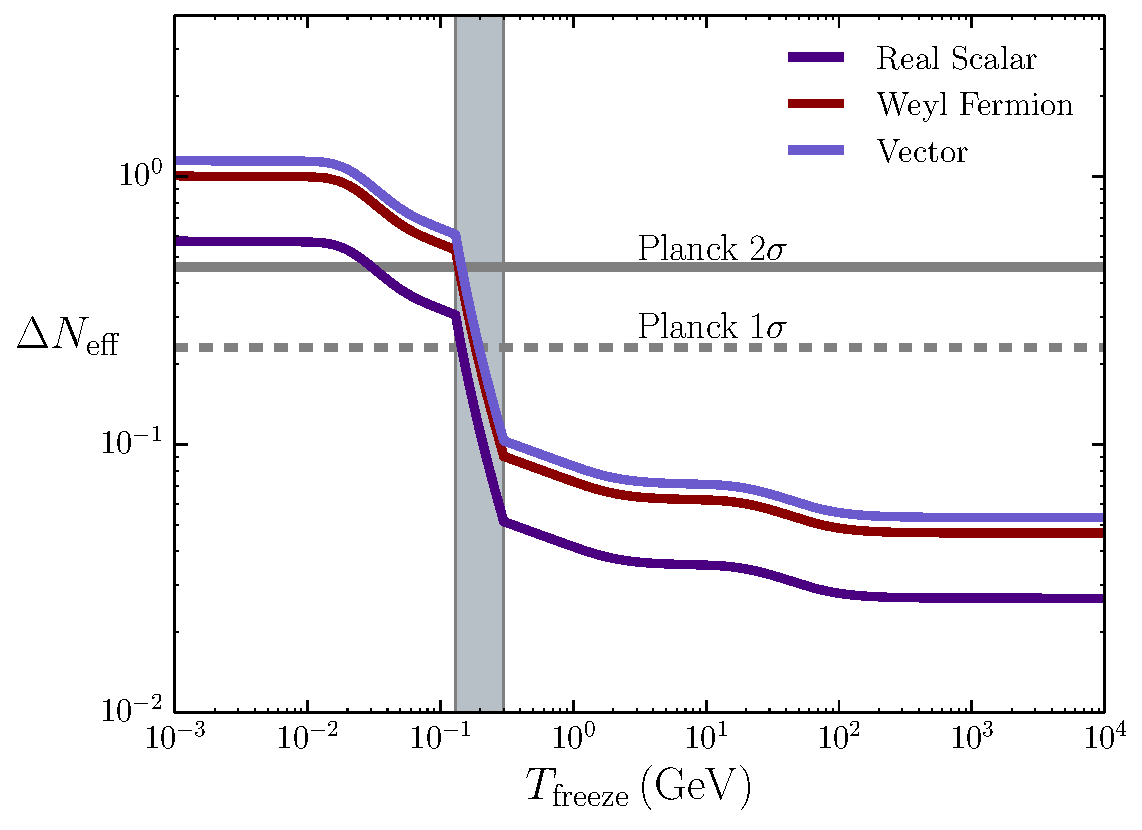
\includegraphics[width=0.65\textwidth]{Neutrinos/Neff.pdf}
\caption{Contribution to $\Neff$ from a massless field that was in thermal equilibrium with the Standard Model at temperatures $T> T_{\rm freeze}$.  For $T_{\rm freeze} \gg m_{\rm top}$, these curves saturate with $\Delta \Neff > 0.027$.   The dashed and solid grey lines correspond to the 1$\sigma$ and 2$\sigma$ sensitivity of Planck, using $\sigma(\Neff) = 0.23$. Temperatures in the grey region correspond to the QCD phase transition.}
\label{fig:Neff_thermal}
\end{center}
\end{figure} 

The contributions to $\Neff$ from hot thermal relics are relatively easy to understand from the discussion of neutrino decoupling in Section~\ref{ThermalHistory}.  After freeze-out, the temperature of a relativistic specifics redshifts like $a^{-1}$ and therefore is only diluted relative to photons when energy is injected.  The annihilation of heavy Standard Model particles into light Standard Model Particles conserves the comoving entropy of the plasma and therefore, the diluted temperature of a relic before neutrino decoupling is given by
\beq
%\left( \frac{T_{\rm relic}}{T_{\nu}} \right)^3 = \frac{g_\star (T_{\nu-{\rm freeze-out}})}{g_\star (T_{\rm relic \, freeze-out}) }= \frac{43/4}{g_\star (T_{\rm freeze-out})} *{jm: Changed g* to \mathcal{N} to match notation from above}
\left( \frac{T_{\rm relic}}{T_{\nu}} \right)^3 = \frac{\gs^{\nu \, {\rm freeze-out}}}{\gs^{\rm relic \, freeze-out} }= \frac{43/4}{\gs^{\rm relic \, freeze-out}} \, ,
\eeq
where $\gs$ is defined as in Section~\ref{ThermalHistory} to be the number of independent spin states including an additional factor of $\frac{7}{8}$ for fermions.  The order of magnitude difference in $\Delta \Neff$ before and after the QCD phase transition comes from an order of magnitude drop in $\gs$ below the QCD scale.  At temperatures well above to top mass, the Standard Model gives $\gs = 106.75$.  

Even a measurement of $\Nf$ which agrees with the Standard Model prediction to high precision would be very interesting due to the constraints it would place on physics beyond the Standard Model.  Some specific implications for sterile neutrinos, axions, and other popular models will be discussed below.  Broadly speaking, constraining $\Delta \Neff$ at the $10^{-2}$ level would constrain or rule out a wide variety of models that are consistent with current cosmological, astrophysical, and lab-based constraints.  Furthermore, because of the sharp change in $\Delta \Neff$ at the QCD phase transition, the improvement from current constraints to projections for CMB-S4 can be quite dramatic.

For the minimal scenario of a single real scalar, reaching $\sigma(\Neff) \sim 1\times 10^{-2}$ would push the constraint on freeze-out temperatures from electroweak scale to the reheat temperature.  This broad reach to extremely high energies and very early times demonstrates the discovery potential for a precision measurement of $\Nf$ with the CMB.  Furthermore, the CMB power spectrum has the ability to distinguish among certain types of dark radiation based on the behavior of its density perturbations  \cite{Chacko:2015noa,Baumann:2015rya}.  This point will be discussed further below.

A measurement with a slightly larger error on $\Nf$ would still be extraordinarily valuable for higher spin fields, multiple light scalars, and modifications to the thermal history up to the electroweak scale.  In particular, massless fermions and vectors have two helicity states which imply contributions of $\Delta \Neff  \geq 0.047$ and $\Delta \Neff  \geq 0.054$ respectively.  As a result, a less sensitive instrument is still capable of probing physics back to reheating since it could detect or rule out the existence of light thermal relics with non-zero spin.  In addition, there is good reason to think dark sectors could contain multiple light fields which could appear at any level of $\Delta \Neff$ above the minimum contribution from a single scalar field.  Still, the most dramatic jumps in discovery potential occur at the critical values $\Delta \Neff = 0.027, 0.047$, and $0.054$.  

\subsection{Observational Signatures}\label{sec:Neffsignatures}

Cosmic neutrinos and other light relics play to two important roles in the CMB that are measured by $\Neff$.  They contribute to the total energy in radiation which controls the expansion history and, indirectly, the damping tail of the power spectrum.  The fluctuations of neutrinos and any other free streaming radiation also produces a constant shift in the of phase the acoustic peaks.  These two effects drive both current and future constraints on $\Neff$.  

The effect of neutrinos on the damping tail drives the constraint on $\Neff$ in the CMB in $\Lambda$CDM + $\Neff$.  The largest effect is from the mean free path of photons, which introduces a suppression $e^{-(k/k_d)^2}$ of short wavelength modes, with~\cite{Zaldarriaga:1995gi}
\beq
k_d^{-2} =\int \frac{da}{a^3 \sigma_T n_e H} \frac{R^2+ \frac{16}{15}(1+R)}{6(1+R)^2} \ ,
\eeq
where $R$ is the ratio of the energy in baryons to photons, $n_e$ is the density of free electrons, and $\sigma_T$ is the Thompson cross-section.  The damping scale is sensitive to the energy density in all radiation through $H \propto \sqrt{\rho_{\rm radiation}}$ during radiation domination (which is applicable at high $\ell$), and is therefore sensitive to $\Neff$ or any form of dark radiation.  From this discussion, we can also see the origin of the degeneracy between $\Neff$ and $n_e$ which may be altered by the primordial helium fraction, $Y_p$.

In reality, the effect on the damping tail is subdominant to the change to the scale of matter radiation equality and the location of the first acoustic peak~\cite{Hou:2011ec}.  As a result, the effect of neutrinos on the damping tail is more accurately represented by holding the first acoustic peak fixed.  This changes the sign of the effect on the damping tail, but the intuition for the origin of the effect (and degeneracy) remains applicable.

In addition to the effect on the Hubble expansion, perturbations in neutrinos affect the photon-baryon fluid through their gravitational influence.  The contributions from neutrinos are well described by a correction to the amplitude and the phase of the acoustic peaks in both temperature and polarization~\cite{Bashinsky:2003tk}.  The phase shift is a particularly compelling signature as it is not degenerate with other cosmological parameters~\cite{Bashinsky:2003tk,Baumann:2015rya}.  This effect is the result of the free-streaming nature of neutrinos that allows propagation speeds of effectively the speed of light (while the neutrinos are relativistic).  Any gravitationally coupled free-streaming light relics will also contribute to the amplitude and phase shift of the acoustic peaks.

E-mode polarization will play an increasingly important role for several reasons.  First of all, the acoustic peaks are sharper in polarization which makes measurements of the peak locations more precise, and therefore aid the measurement of the phase shift.  The second reason is that polarization breaks a number of degeneracies that would also affect the damping tail~\cite{Baumann:2015rya}.

{\it Status of current observations} -- Planck has provided a strong constraint on $\Neff = 3.15 \pm 0.23$ when combining both temperature and polarization data.  The addition of polarization data has both improved the constraint on $\Neff$ and reduced the impact of the degeneracy with $Y_p$.  Recently, the phase shift from neutrinos has also been established directly in the Planck temperature data~\cite{Follin:2015hya}.  This provides the most direct evidence for presence of free-steaming radiation in the early universe, consistent with the cosmic neutrino background.


\subsection{Forecasts}\label{sec:neff_forcast}

As we described in Section~\ref{sec:Neffsignatures}, the most concrete signatures of $\Neff$ from CMB-S4 are derived from the damping tail at high-$\ell$ in both $T$ and $E$.  In addition, there is the effect of the shift in the phase of the acoustic peaks that is present at $\ell > 500$.  Within $\Lambda$CDM these parameters are robust to degeneracies, having already accounted for the degeneracy of the location of the first acoustic peak with $H_0$.  The damping tail is degenerate with other extensions, like $Y_p$, as we will explore in Section~\ref{sec:NeffBBNfore}.

Forecasts for $\sigma(\Neff)$ under various experimental configurations are given in Table~\ref{tab:Neffbeam}.  Since the damping tail extends to very high-$\ell$, constraints on $\Neff$ are sensitive to $\ell_{\rm max}$ and the beamsize of the experiment.  We assume $\ell_{\rm max} = 5000$ except for $C^{TT}_{\ell}$ where we assume $\ell_{\rm max} = 3000$ due to foregrounds.  One can see the impact of the highest-$\ell$ modes  by looking at the effect of the beamsize.

The other important parameter for $\Neff$ is the sky fraction of the survey, $f_{\rm sky}$.  Since the signature of neutrinos depends on the detailed measurement of the shape of the power spectra, constraints depend on the number of observed modes.  At fixed noise levels this implies that $\sigma(\Neff) \propto f^{-1/2}_{\rm sky}$.  Of course, with a fixed number of detectors the sensitivity, $S$, is proportional to $S \propto f_{\rm sky}^{1/2}$.  Since $\sigma(\Neff)$ grows more slowly than $S$, we see that there is a net improvement in $\sigma(\Neff)$ by increasing $f_{\rm sky}$ at a fixed number of detectors.  This trend is shown in Figure~\ref{fig:Neff_fsky}.


\begin{table}[t!]
\begin{center}
\begin{tabular}{l ccc} 
 \toprule
    		sensitivity / beamsize	    			& $1'$  		& $2'$  		& $3'$  		 \\ [0.5ex]
 \midrule
   1 $\mu$K-arcmin & 0.030 		& 0.032		& 0.35	 		  \\
  2  $\mu$K-arcmin & 0.035 		& 0.038		& 0.041	 		  \\
   3  $\mu$K-arcmin & 0.040 		& 0.042 		& 0.045	 		  \\
    \bottomrule
\end{tabular}
\caption{Forecasts for $\sigma(\Neff)$ with varying beamize in arcmin (') and detector sensitivity.  These forecasts assume $f_{\rm sky} = 0.4$.  }
\label{tab:Neffbeam}
\end{center}
\end{table}


\begin{figure}[t!]
\begin{center}
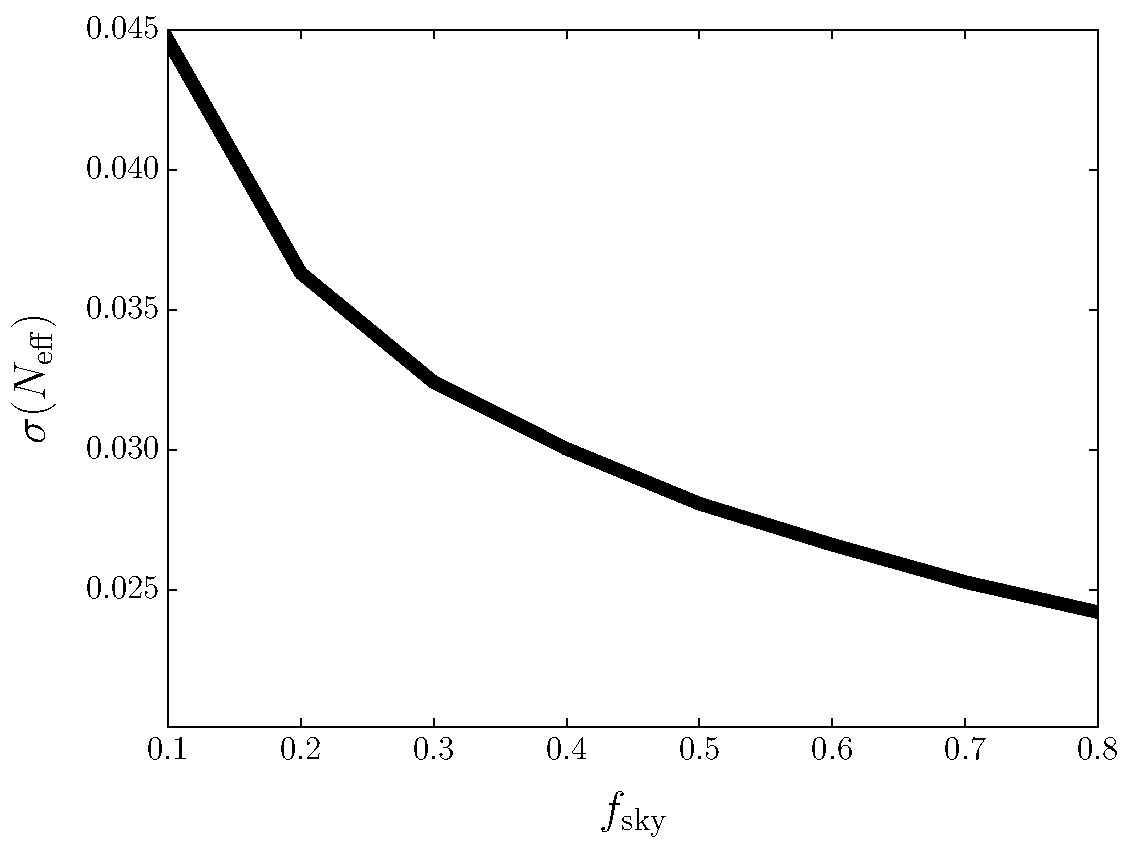
\includegraphics[width=0.65\textwidth]{Neutrinos/Nfsky.pdf}
\caption{Forecasts for $\sigma(\Neff)$ as a function of sky fraction.  The sensitivity have been normalized to 1 $\mu$K-arcmin for $f_{\rm sky} =0.4$ and is scaled according to $S \propto f_{\rm sky}^{1/2}$ for different sky fractions.  The grey line shows that value of $\sigma(\Neff) =0.027$ which is the 1$\sigma$ sensitivity any scalar thermal relic, or equivalently, 2$\sigma$ sensitivity to any vector thermal relic.  For a fixed number of detectors, we see that $\sigma(\Neff)$ is minimized by increasing sky fraction.  }
\label{fig:Neff_fsky}
\end{center}
\end{figure} 


We see from these results that for sufficiently large sky fraction, the thresholds for the light fermions and vectors are accessible at 2$\sigma$ for plausible experimental configurations, or equivalently, 1$\sigma$ for the minimum threshold for a light scalar.  Specifically, we can reach $\sigma(\Neff) = 0.027$ with $S = 1$ $\mu$K-arcmin using 1' beams or 2' beams for $f_{\rm sky} \geq 0.5$ and $f_{\rm sky} \geq 0.6$ respectively.  Reaching at least 2$\sigma$ sensitivity for the light scalar may be possible with more extreme design configurations (i.e. lower noise at large sky fraction).  In Figure~\ref{fig:Neff_S4_thermal}, we show how 2$\sigma$ limits available with CMB-S4 translate into limits on the freeze-out temperature of a single additional species.  While Planck is only sensitive to physics after the QCD phase transition (Figure~\ref{fig:Neff_thermal}), CMB-S4 can reach times before the QCD phase transition for all spins, and back to reheating for spins 1/2 and 1.  

These results are tantalizingly close to some exciting theoretical targets.  This raises the question of whether we can reach these targets at higher significance by other means.  First, constraints on $\Neff$ improve significantly if $\ell_{\max}^{TT} > 3000$.  These modes are currently ignored due to foregrounds, but foreground removal could make some of the modes accessible.  Second, one could also imagine the sensitivity could be improved in combination with large scale structure surveys such as DESI and LSST, both by breaking degeneracies and providing a future measurement of the power spectrum.  

\begin{figure}[t!]
\begin{center}
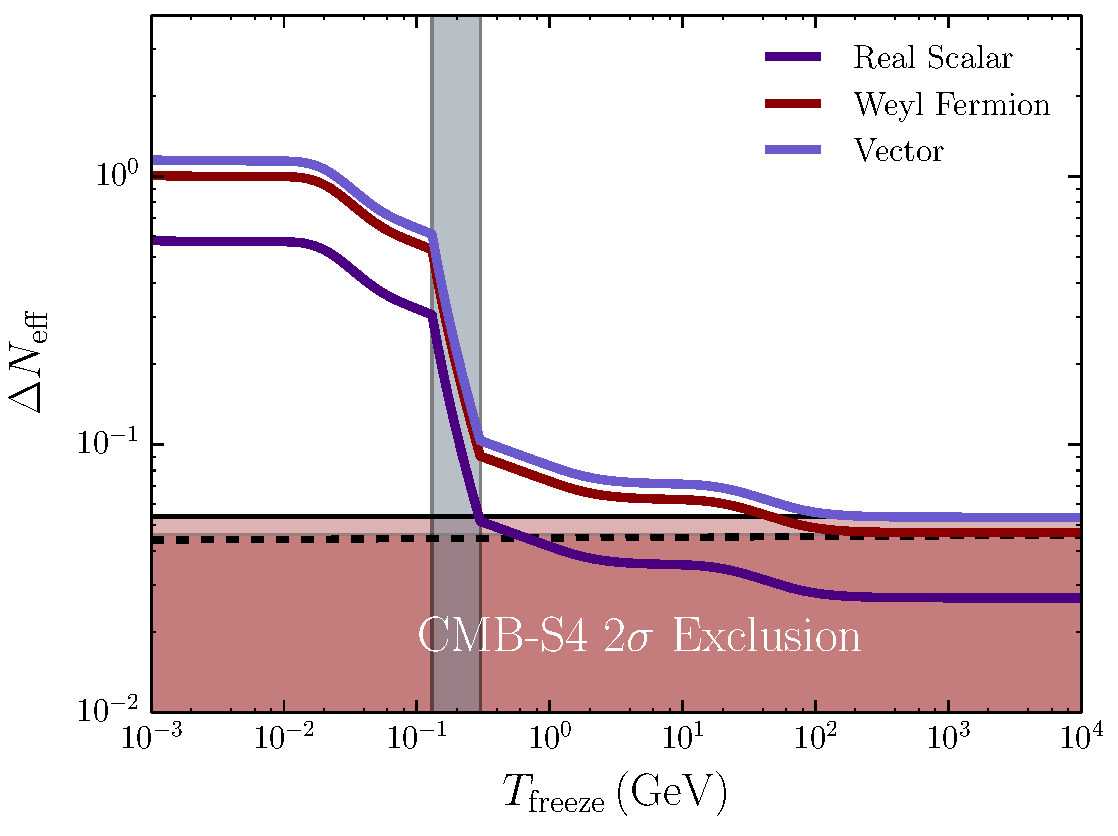
\includegraphics[width=0.65\textwidth]{Neutrinos/Neff_S4.pdf}
\caption{Same as Figure~\ref{fig:Neff_thermal} showing plausible 2$\sigma$ limits from CMB-S4 in red, assuming 1' beams and 1 $\mu$K-arcmin temperature noise.  The light red region with solid boundary and darker red with dashed boundary are for $f_{\rm sky}=0.5$ and $f_{\rm sky} =0.7$ respectively.}
\label{fig:Neff_S4_thermal}
\end{center}
\end{figure} 



\section{Implications for Light Particles}\label{sec:BSMneff}

Contributions to $\Delta \Neff$ from light particles depends sensitively on the spin.  For thermal relics, each degree of freedom contributes equally, so the signatures scale like the effective degrees of freedom of a given particle.  In addition, the couplings that would thermalize these particles depend both on the spin of the particle and the spin of the particle(s) it couples to in the Standard Model.  Furthermore, these couplings can be non-thermal production mechanisms that also contribute to $\Delta \Neff$. This section explores the implications of a CMB-S4 measurement of $\Neff$ for a number of well motivated models, organized by the spin of the relevant light particle from axions (spin 0) to gravitons (spin 2).  

\subsection{Axions}
\label{sec:neffaxions}

Light particles of spin-0 (scalar fields) are highly constrained by naturalness.  In the absence of a symmetry, one would expect them to be heavy and thus a poor candidate for dark radiation.  On the other hand, (pseudo) Goldstone bosons are naturally light and they appear generically from spontaneous breaking of some high energy global symmetry.  A ubiquitous  example in Beyond the Standard Model physics are axions and/or axion-like particles (ALPs).  Axions have been introduced to solve the strong-CP problem~\cite{Peccei:1977hh}, the hierarchy problem~\cite{Graham:2015cka}, and the naturalness of inflation~\cite{Freese:1990rb}.  Furthermore, they appear generically in string theory, in large numbers, leading to the qualitative phenomena described as the string axiverse~\cite{Arvanitaki:2009fg}.  They may even be tied to the origin of the breaking of the flavor and baryon/lepton number symmetries of the Standard Model.

At low energy, the mass of the ALP is protected by an approximate shift symmetry of the general form $a \to a + c$ where $a$ is the axion and $c$ is a constant (for non-abelian Goldstone bosons, this transformation will include higher order terms in $a$).  We will define an ALP to be any such particle where all of the couplings of the axion to the Standard Model respect such a symmetry.  This symmetry may be softly broken with an explicit mass term, although this is highly restricted in the case of the QCD axion.


%\subsubsection{Constraints on Axion couplings}\label{sec:axionbsm}

%A ubiquitous component of extensions of the Standard Model are axions and/or axion-%like particles (ALPs).  Axions have been introduced to solve the strong-CP problem~%\cite{Peccei:1977hh}, the hierarchy problem~\cite{Graham:2015cka}, and the %naturalness problem of inflation~\cite{Freese:1990rb}.  Furthermore, they appear %generically in string theory in large numbers, leading to the qualitative phenomena %described as the string axiverse~\cite{Arvanitaki:2009fg}.

%ALPs typically appear as (pseudo)-Goldstone bosons of some high energy global %symmetry.  At low energy, the mass of the ALP is protected by an approximate shift %symmetry of the general form $a \to a + c$ where $a$ is the axion and $c$ is a %constant (for non-abelian Goldstone bosons, this transformation will include higher %order terms in $a$).  We will define an ALP to be any (pseudo)-scalar particle for %which all couplings to the Standard Model respect such a symmetry.  This symmetry %may be softly broken with an explicit mass term, although this is highly restricted %in the case of the QCD axion.

Two very common features of models containing ALPs are that the ALPs are typically light (in many cases, $m \ll 1$~eV) and their interactions are suppressed by powers of the (typically large) decay constant $f_a$.  These two features make ALPs a particularly compelling target for cosmology and $\Neff$ specifically~\cite{Brust:2013xpv,Salvio:2013iaa,Kawasaki:2015ofa,Baumann:2016wac}.  Because of their small masses, ALPs will often behave as relativistic species in the early universe.  Furthermore, because their production rate will scale as $T^{2n +1} / f_a^{2n}$ for some $n \geq 1$, they are likely to be thermalized at high temperatures.  Given that $\Delta \Neff > 0.027$ under such circumstances, a CMB experiment with sensitivity at this level will be sensitive to a very wide range of ALP models.   In the absence of a detection of $\Delta \Neff$, we can place constraints on the axions couplings to the Standard Model.  

Two couplings of particular interest for axion phenomenology are the coupling to gluons and photons, 
\beq
\frac{1}{4} g_{a \gamma \gamma} a \tilde F_{\mu \nu}F^{\mu\nu} \ , \qquad \qquad \frac{1}{4} g_{a g g} a \tilde G_{\mu \nu}G^{\mu\nu}  \ .
\eeq
These couplings typically appear as the consequence of chiral anomalies.  The coupling of the axion to gluons is what makes the solution to the strong-CP problem possible.  The coupling to photons is somewhat model dependent but typically arises in conjunction with the gluon coupling.  In addition to or instead of these couplings, a variety of other possible couplings to matter may also be included.

\begin{figure}[h!]
\centering 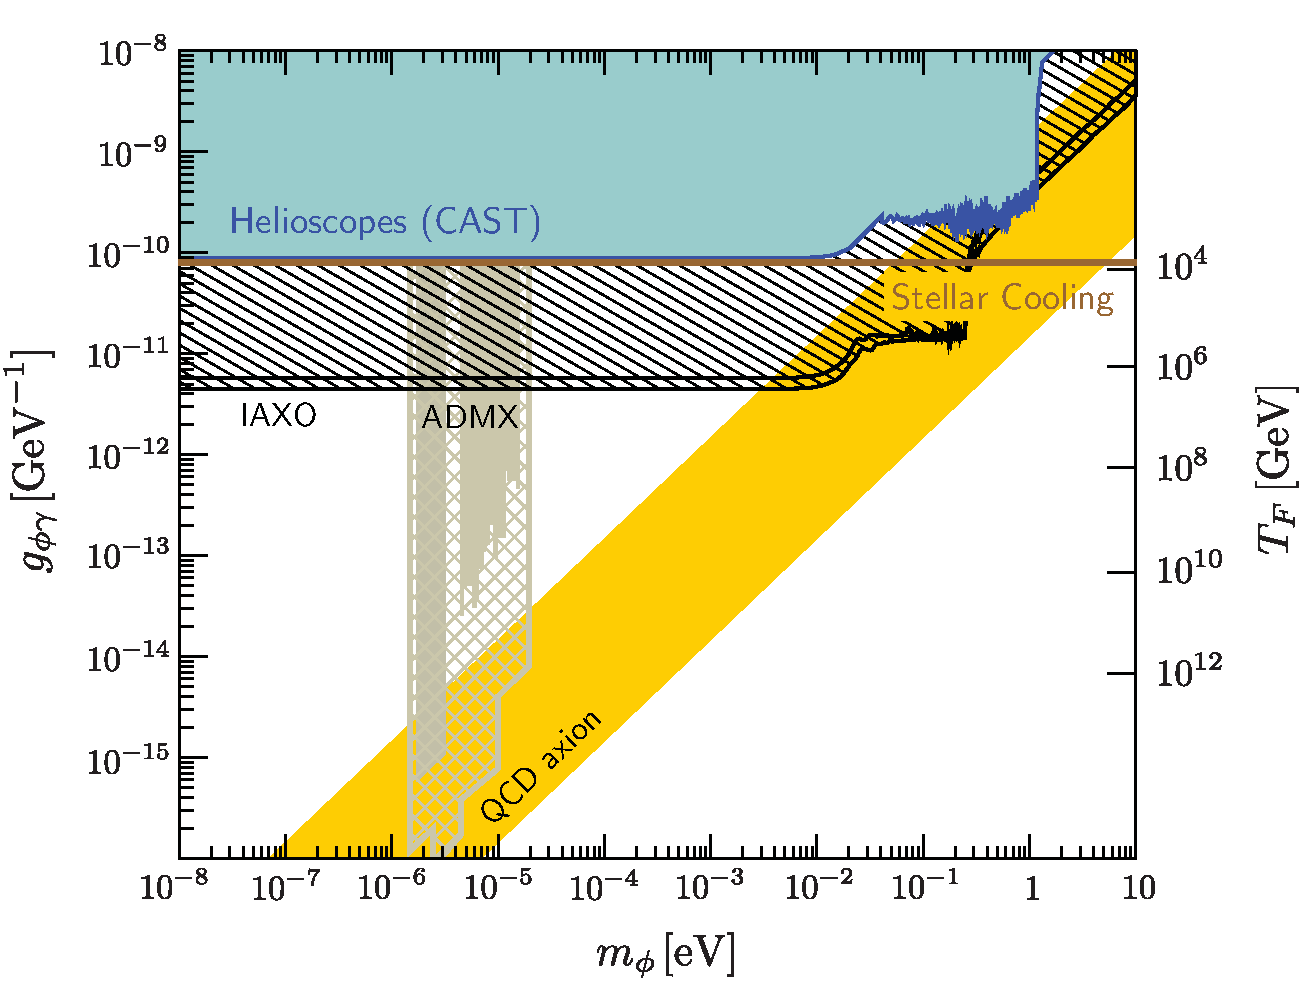
\includegraphics[width=0.70\textwidth]{Neutrinos/AxionPhotonWithFuture.pdf}
\caption{Relationship between freeze-out temperature ($T_F$) and axion-photon coupling ($g_{a\gamma\gamma}$).  While freeze-out is independent of the mass, experimental probes of the coupling are strongly mass dependent.  For $T_F > 10^4$~GeV the axion coupling would predict $\Delta \Neff = 0.027$.  Sensitivity to $\Delta\Neff$ at that level would translate into sensitivity to axions with $T_F \leq T_{\rm reheat}$.  For plausible values of $T_{\rm reheat} > 10^{10}$~GeV, cosmology is orders of magnitude more sensitive than existing bounds over a wide range of masses.}
\label{fig:axionphoton}
\end{figure}



The coupling of axions to matter has an additional feature that it can bring axions into thermal equilibrium at high temperatures.  Specifically, the lowest-dimension coupling of an axion to charged matter takes the form
\beq
{\cal L} = -\frac{\partial_\mu a}{\Lambda_\psi}  \bar \psi_i ( \gamma^\mu g^{ij}_V + g_A^{ij} \gamma^5 ) \psi_j
\eeq
where $\psi_{i}$ is any of the charged fermions of the Standard Model and $i,j$ label the three generations of fermions of with the same charges.  Above the scale of electroweak symmetry breaking (EWSB), this coupling leads to an abundance of axions with $\Delta \Neff = 0.027$.  Through freeze-out, we are again very sensitive to $g_V$ and $g_A$ at levels that vastly exceed current limits.  In addition, below the scale of EWSB, this coupling can bring the axions into thermal equilibrium at low temperatures (freeze-in) below the mass of the heaviest fermion, $T_F \lesssim m_{3}$.  Freeze-in will produce $\Delta \Neff \approx 0.05$ and is therefore easier to detect.  For reheating temperatures well above the electroweak scale, the sensitivity of freeze-out exceeds that of freeze-in, although both are far more sensitive than current limits on axion couplings to  second and third generation fermions.

The coupling to matter is motivated also by the approximate $U(3)^5$ flavor symmetry of the Standard Model.  It is natural for such couplings to arise if the axion is a goldstone boson that results from spontaneous breaking of this symmetry (or a sub-group).  Given the non-abelian nature of the flavor symmetry, these scenarios can often lead to many axions (also known as familons).  Under such circumstances, the contribution to freeze-out is given by 
\beq
\Delta \Neff = N_a \times 0.027
\eeq
where $N_a$ is the number of axions / number of broken generators of the symmetry group.  It is easy to find scenarios where $N_a\sim {\cal O}(10)$ which is at the current level of sensitivity.


{\it Status of current observations} -- Current constraints on ALPs arise from a combination of experimental~\cite{Graham:2015ouw}, astrophysical~\cite{Raffelt:2012kt}, and cosmological~\cite{Marsh:2015xka} probes.  Current cosmological constraints are driven by several effects that depend on the mass of the axion.  For axion masses greater than 100 eV, stable thermal ALPs are easily excluded because they produce dark matter abundances inconsistent with observations.  By including the free-streaming effects of thermal QCD-axions,  Planck data~\cite{DiValentino:2015wba} combined with local measurements provide the constrain $m_a < 0.525$ eV (95 \% CL).  At larger masses, ALPs become unstable and can be constrained by the change to $\Neff$ from energy injection as well as from spectral distortions and changes to BBN~\cite{Cadamuro:2011fd,Follin:2015hya}.

{\it Implications for CMB Stange IV} -- Sensitivity to $\Delta \Neff =0.027$ is sufficient to probe the entire mass range of ALPs down to $m_a =0$ under the assumption that they thermalized in the early universe.  Interpreting such bounds in terms of the couplings of axions is more complicated~\cite{Brust:2013xpv} and can depend on assumptions about the reheating temperature.  For high (but plausible) reheat temperatures of $10^{10}$ GeV, CMB stage IV would be sensitive to $g_{a\gamma \gamma}, \, g_{a g g} \,  < \, 10^{-13} {\rm GeV}^{-1}$~\cite{Baumann:2016wac} as illustrated in figures~\ref{fig:axionphoton} and~\ref{fig:axiondipole}.  These projected limits exceed current constraints and future probes for a range of possible axion masses (including the QCD axion).

The implications for the couplings to matter are similar for the contribution from freeze-out.  However, the freeze-in contribution of $\Delta \Neff \gtrsim 0.05$ would be easier to exclude experimentally, but still produces the limits~\cite{Baumann:2016wac}
\beq
\Lambda_{\psi_i}  \ >\ \left\{ \begin{array}{ll} \displaystyle 1.3\times 10^8 \, {\rm GeV} \left(\frac{g_{*,i}}{g_{*,\tau}}\right)^{\!-1/4} \left(\frac{m_i}{m_\tau}\right)^{\!1/2} & \quad i=\text{leptons}, \\[10pt]
\displaystyle 2.1\times 10^9 \, {\rm GeV} \left(\frac{g_{*,i}}{g_{*,t}}\right)^{\!-1/4} \left(\frac{m_i}{m_t}\right)^{\!1/2} & \quad i=\text{quarks}.
\end{array} \right.
\eeq
where $g_{*,i}$ is the number of degrees of freedom at temperature $T = m_i$.  For second and third generation fermions, these limits would exceed current bounds by several orders of magnitude.


\begin{figure}[h!]
\centering 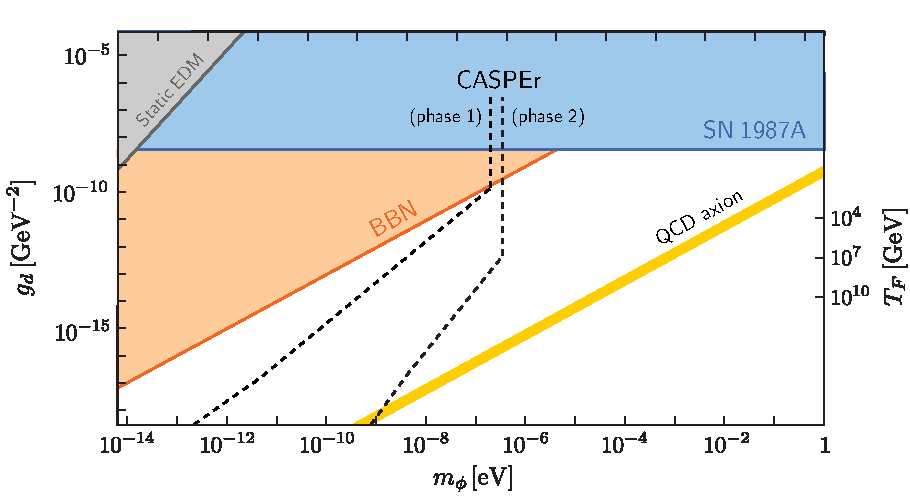
\includegraphics[width=0.70\textwidth]{Neutrinos/DipoleWithCASPErAndBBN.pdf}
\caption{Relationship between freeze-out temperature ($T_F$) and axion-gluon coupling via the neutron dipole ($g_d$).  While freeze-out is independent of the mass, experimental probes of the coupling are strongly mass dependent. We see that cosmology is more sensitive than current limits even for freeze-out temperatures below the eletro-weak phase transition and therefore could be probed by $\Delta \Neff > 0.027$.   }
\label{fig:axiondipole}
\end{figure}




%Two very common features of these models are that the axions are typically light (in many cases, $m \ll 1$ eV) and their interactions are suppressed by powers of $f_a$, the dimensional scale that controls the symmetry breaking.  These two features make ALPs a particularly compelling target for $\Neff$.  Because of the small masses, they will often behave as relativistic species in the CMB.  Furthermore, because their production rate will scale as $T^{2n +1} / f_a^{2n}$ for some $n \geq 1$, they are likely to be thermalized at high temperatures.  Given that $\Delta \Neff \geq 0.027$ under such circumstances, a CMB experiment with sensitivity at this level will be sensitive to a very wide range of ALP models.

%A CMB experiment sensitive to $\Delta \Neff \leq 0.027$ would have a dramatic impact on axion physics.  We provide a detailed discussion of the constraints on individual couplings in Section~\ref{sec:axionbsm}, but here we will illustrate the impact qualitatively.  At this sensitivity, any freeze-out at $T< T_{\rm reheat}$ would be detectable in the CMB since they would all produce $\Delta \Neff$.  Since freeze-out is controlled by $f_a$ we can translate the measurements of $\Neff$ into limits on $f_a$.  Since it is possible that $T_{\rm reheat} >10^{10}$ GeV, freeze-out is generally sensitive to $f_a$ as high as $10^{12-14}$ GeV.  This easily surpasses the sensitivity from stellar cooling ($f_a \lesssim 10^{10}$ GeV), which to date is one of the most broadly sensitive probes of axions.  As long as $T_{\rm reheat} > 10^{4}$ GeV, the CMB will be a more sensitive than stellar cooling to these models.

%Axions can also produce $\Delta \Neff> 0.027$ in a wide variety of well-motived circumstances.  A case of particular interest is when axions couple directly to Standard Model fermions.  The Standard Model has an $U(3)^5$ flavor symmetry and it is for axions couplings to arise if the axion is a goldstone boson that results from spontaneous breaking of this symmetry (or a sub-group).  Given the non-abelian nature of the flavor symmetry, these scenarios can ofter lead to many axions (also known as familons).  Under such circumstances, the contribution to freeze-out is given by 
%\beq
 %\Delta \Neff = N_a \times 0.027
 %\eeq
 %where $N_a$ is the number of axions / number of broken generators of the symmetry group.  It is easy to find scenarios where $N_a\sim {\cal O}(10)$ which is at the current level of sensitivity.
 


\subsection{Light Fermions and Vectors}

A general approach to interpreting $\Neff$ constraints in terms of massless fields of arbitrary spin was undertaken in~\cite{Brust:2013xpv}.  One identifies the symmetry that is required to explain  the small mass of the particle, and then writes the most general interactions with the Standard Model consistent with the symmetry.  The couplings will take the form
\beq
{\cal L} \supset \sum_{\Delta_h, \Delta_s} \frac{1}{\Lambda^{\Delta_h+ \Delta_s-4}} \,  {\cal O}_{h, \Delta_h} \cdot {\cal O}_{s, \Delta_s}
\eeq
where ${\cal O}_{h,\Delta_h}$ is an operator of dimension $\Delta_h$ constructed only from hidden sector fields (and similarly for ${\cal O}_{s, \Delta_s}$ and Standard Model fields).  The total operator must be a scalar under both the Lorentz transformations and the symmetry that protects the mass of the hidden sector field(s).  The bounds on axions discussed in Section~\ref{sec:neffaxions} are one such example, where the axion is protected by a shift symmetry.  For the purpose of this discussion, we have classified all scalars of this type as axions.

For a single Weyl fermion, $\chi$, the leading couplings to the Standard Model are through the anapole moment and four-fermion interactions
\beq
{\cal L} \supset \frac{\chi^{\dagger} \bar \sigma^{\mu} \chi}{\Lambda_{\chi}^2} \Big( d_a  \, \partial^\nu F_{\mu \nu} + d_f \,  \bar \psi \gamma_\mu \psi \Big) \ ,
\eeq
where we have chosen a chosen one of several four-fermion interactions for illustration and $d_f, d_a$ are order one numbers.  Current experimental constraint from LEP and the LHC limit $\Lambda_\chi \gtrsim \, 1$ TeV.  Similar bounds are set by Planck by excluding the contributions to $\Delta \Neff$ from freeze-out after the QCD phase transition.  If we are sensitive to the minimal contribution from a Weyl fermion of $\Delta \Neff = 0.047$, then for a reheat temperature of $T_{\rm reheat} \sim 10^{10}$ GeV, we would be sensitive to $\Lambda_\psi \lesssim 10^{12}$ GeV.  We see that for an order of magnitude improvement in sensitivity to $\Neff$, we get as much as a nine order of magnitude improvement in sensitivity to $\Lambda_\psi$.  

For a hidden Dirac fermion with a $U(1)$ global symmetry, $X$, the leading\footnote{The dipole operator preserves the same $U(1)$ symmetry that allows a Dirac mass.  It is unclear if one can UV-complete this model with a small Dirac mass.} coupling is through an effective dipole interaction.  A similar interaction also permits a hidden $U(1)$ gauge boson, $A'_\mu$, to couple to Standard Model fermions.
\beq
{\cal L} \supset  \frac{1}{\Lambda_X} \bar X \sigma_{\mu\nu} X  F^{\mu \nu} + \frac{1}{\Lambda_{A'}^2} H \bar \psi \sigma_{\mu\nu} \psi  F'_{\mu \nu}  \ ,
\eeq
where $F'_{\mu \nu}$ is the field strength of $A'_\mu$.  The We have included the Higgs field, $H$, in the coupling to Standard Model fermions as it is required by gauge invariance above the scale of EWSB.  Stellar cooling provides a strong constraint of $\Lambda_X \gtrsim 10^9$ GeV and $\Lambda_{A'} \gtrsim 10^5$ GeV.  

Freeze-out above the scale of EWSB for a Dirac fermion produces $\Delta \Neff = 0.094$ and $\Delta\Neff = 0.054$ for a hidden photon.  For a reheating temperature of $10^{10}$ GeV, we are sensitive to $\Lambda_X \lesssim 10^{13}$ GeV and $\Lambda_{A'}  \lesssim 10^{11}$ GeV respectively.  The Dirac fermion will be accessible with CMB-S4 and will improve on the stellar cooling constraint for a reheat temperature $T_{\rm reheat} > 10^4$ GeV.

\subsection{Gravitinos}

One of the most popular extensions of the Standard Model is supersymmetry, which is motivated both by naturalness and gauge coupling unification.  Although the most generic possibilities are under significant tension for the LHC, there are still a variety of possibilities consistent with low-scale supersymmetry.

One of the universal predictions of supersymmetry is the existence of a spin-3/2 partner to the graviton, the gravitino.  The gravitino mass is determined by the absolute scale of supersymmetry breaking, 
\beq
m_{\frac{3}{2}} = \frac{|F|}{\sqrt{3} M_{\rm pl}}
\eeq
where $|F|$ is the order parameter for the scale of SUSY breaking (the vacuum expectation value of the auxiliary field $F$).  This result does not depend on details of the mechanism of SUSY breaking unlike the super-partners of the rest of the Standard Model particles.

The typical coupling strength of the gravitino is the same as the graviton, $8 \pi G = \Mpl^{-2}$.  However, the strength of the coupling to the helicity-1/2 component of the gravitino is enhanced by $\Mpl^2 /F$.  This is simply the statement that the goldstino of SUSY breaking is coupled with strength $F^{-1}$ (but is `eaten' by the gravitino).  Due to the enhanced coupling, the gravitino can be in thermal equilibrium with the Standard Model at plausible temperatures in the early universe.  The gravitino therefore behaves just like a Weyl fermion in figure~\ref{fig:Neff_thermal}.

For $m_{3/2} \lesssim 10$ eV, hot relic gravitinos free stream on the scale of the CMB and therefore lead to observable signatures.  Current data from Planck already requires that $m_{3/2} < 4.7$ eV from a combination of the primary CMB and CMB lensing~\cite{Osato:2016ixc}.  To probe lower masses, note that for $m_{3/2} < {\cal O}(1)$ eV a gravitino will behave as free-streaming radiation from the point of view of the CMB.  One finds that for these low values of the mass, gravitinos contribute a shift to $\Neff$,
\beq
\left(\Delta \Neff\right)_{3/2} \, \gtrsim \, 0.057 \ .
\eeq
This number is somewhat larger than the minimum value of $\Delta \Neff =0.047$ for the helicity-1/2 component because the effective compiling becomes large as $m_{3/2} \to 0$.  As a result for $m_{3/2} < 1$ eV, the gravitinos decouple below 100 GeV.  At $\sigma(\Neff) \sim 0.03$, CMB-S4 can rule out all low-scale SUSY breaking models allowed by current cosmology.  

\subsection{Gravitational Waves}\label{sec:constraintsntNeff}

Since gravitational waves are massless and free-streaming, any gravitational waves which were present in the early universe naturally contribute to the total radiation energy density, and can therefore be constrained with $\Neff$ \cite{Boyle:2003km,Boyle:2007zx,Stewart:2007fu,Meerburg:2015zua,Lasky:2015lej}.

Let us briefly review how to compute the energy density of a stochastic background of gravitational waves, following the treatment of \cite{Isaacson:1968zza,Misner:1974qy,Watanabe:2006qe,Maggiore:1900zz}.  We will take the metric of spacetime to be given by a background component $\bar{g}_{\mu}$ described by the flat Friedmann-Robertson-Walker metric and a perturbation $\delta g_{\mu\nu}$.  We will take the characteristic frequency of $\delta g_{\mu\nu}$ to be much higher than that of $\bar{g}_{\mu\nu}$.  In particular, we will focus on gravitational waves whose wavelengths are much shorter than scales of cosmological interest.

The Ricci tensor can be expanded in powers of $\delta g$ as
\begin{equation}\label{eq:Ricci_GW}
	R_{\mu\nu} = \bar{R}_{\mu\nu} + R_{\mu\nu}^{(1)} + R_{\mu\nu}^{(2)} + \cdots \, .
\end{equation}
We are interested in determining how spacetime is curved by the presence of small scale gravitational waves, or in other words, how $\bar{R}_{\mu\nu}$ is affected by terms containing $\delta g_{\mu\nu}$.  Since $R_{\mu\nu}^{(1)}$ is linear in $\delta g_{\mu\nu}$, it contains only high frequency components, while on the other hand, $R_{\mu\nu}^{(2)}$ has both low and high frequency parts.  

The high frequency part of Einstein's equations governs how gravitational waves propagate in a curved background, and is not necessary here.  For the low frequency part, we can take an average over several cycles of the high frequency modes, which then gives
\begin{equation}\label{eq:Einstein_Eq_GW}
	\bar{R}_{\mu\nu} = -\left\langle R_{\mu\nu}^{(2)}\right\rangle + 8\pi G \left\langle T_{\mu\nu}-\frac{1}{2}g_{\mu\nu}T\right\rangle \, .
\end{equation}
We can then read off the effective energy-momentum tensor of small scale fluctuations
\begin{equation}\label{eq:EM_Tensor_GW}
	T_{\mu\nu}^\mathrm{GW} = -\frac{1}{8\pi G} \left \langle R_{\mu\nu}^{(2)}-\frac{1}{2}\bar{g}_{\mu\nu}R^{(2)} \right\rangle + \mathcal{O}(\delta g^3) \, .
\end{equation}
If we take our perturbation to be of the form $\delta g_{ij} = a^2 h_{ij}$ with $h_{ij,j} = 0$ and $h_{ii} = 0$, we can compute the energy density of gravitational waves explicitly in the transverse traceless gauge
\begin{equation}\label{eq:Energy_GW}
	\rho_\mathrm{GW} = T_{00}^\mathrm{GW} = \frac{1}{32 \pi G}\delta^{ik}\delta^{j\ell}\left\langle \dot{h}_{ij} \dot{h}_{k\ell} \right\rangle + \mathcal{O}(\delta g^3) \, .
\end{equation}

We will define the gravitational wave power spectrum as
\begin{equation}\label{eq:GW_power_spectrum}
	\left\langle h_{ij}(\eta,\mathbf{x})h^{ij}(\eta,\mathbf{x})\right\rangle \equiv \int  d \log k \, \mathcal{P}_t(k) \left[\mathcal{T}(\eta,k)\right]^2 \, ,
\end{equation}
where $\mathcal{P}_t(k)$ is the primordial power spectrum of gravitational waves and $\mathcal{T}(\eta,k)$ is the tensor transfer function.  The energy density of gravitational waves is then given by
\begin{equation}\label{eq:GW_energy_density}
	\rho_\mathrm{GW} = \frac{1}{32\pi G a^2}\int  d\log k \, \mathcal{P}_t(k) \left[\mathcal{T}'(\eta,k)\right]^2 \, ,
\end{equation}
where the prime denotes a derivative with respect to conformal time $\eta$.

Direct searches for the stochastic gravitational wave backgound are often quoted in terms of the normalized energy density per logarithmic scale
\begin{equation}\label{eq:Omega_GW}
	\Omega_\mathrm{GW}(k) \equiv \frac{8\pi G}{3H_0^2}\frac{d\rho_\mathrm{GW}}{d\log k} = \frac{\mathcal{P}_t(k)}{12H_0^2a_0^2} \left[\mathcal{T}'(\eta_0,k)\right]^2 \, .
\end{equation}
On the other hand, constraints on $\Neff$ provide an integral constraint on the spectrum of gravitational waves since waves of all frequencies contribute to the total energy density.

If for example, we take the primordial gravitational wave power spectrum to be a simple power law of the form $\mathcal{P}_t(k) = A_t \left(\frac{k}{k_\star}\right)^{n_t}$ (as in Eq.~(\ref{eq:power_spectra_power_law})), we can use a constraint on $\Neff$ to place bounds on the tensor spectral tilt $n_t$.  The contribution to $\Neff$ can then be approximated for $n_t>0$ as \cite{Meerburg:2015zua}
\begin{equation}\label{eq:Neff_GW}
	\Delta \Neff \simeq \left(3.046 + \frac{8}{7}\left(\frac{11}{4}\right)^{4/3}\right)\frac{A_t}{24n_t}\left(\frac{k_\mathrm{UV}}{k_\star}\right)^{n_t} \, ,
\end{equation}
where $k_\mathrm{UV}$ represents the ultraviolet cutoff of the primordial tensor power spectrum.  While this constraint does not probe the regime of great interest for inflationary models, it does provide a useful constraint on early universe alternatives to inflation which predict positive tensor tilt.



\section{Complementarity of CMB and BBN}\label{sec:bbn}

%\subsection{Introduction} \label{Introduction}

Primordial light element abundances have for many decades been an interesting observational test of hot big bang cosmology.  The process by which light elements form in the early universe known as big bang nucleosynthesis (BBN) was worked out theoretically in the early days of the development of the hot big bang model of cosmology \cite{Alpher:1948ve}.  It is a process which depends on all four fundamental forces, that unfolded during the first three minutes of our current phase of expansion, and which has long provided a useful constraint on physics beyond the Standard Model.  The current observational inferences of the primordial deuterium and helium abundances are in good agreement with the predictions of standard BBN.  Primordial light element abundances are sensitive to the radiation content of the universe as measured through $\Nf$, which also affects the angular power spectrum of the CMB.  Combining these two probes provides useful insight into the physics of the early universe which neither could achieve alone.

\subsection{Standard Big Bang Nucleosynthesis} \label{StandardBBN}
In this section, we will briefly review the physics of big bang nucleosynthesis in the Standard Model.  For more extensive reviews see for example \cite{Weinberg:2008zzc,Agashe:2014kda,Cyburt:2015mya}.

The salient features of the early universe at the BBN epoch are that: (1) the entropy per baryon is high (baryon-to-photon ratio $6.1\times {10)}^{-10}$); and (2) the expansion rate is driven by gravitation, and is therefore is relatively slow. As a consequence of the latter, at temperatures well above $T \sim 1\,{\rm MeV}$ the strong, electromagnetic, and even the weak interaction are in chemical and thermal equilibrium. As the universe expands and the temperature drops the rates of neutrino scattering processes fall and, eventually, these are so slow that they cannot effect efficient exchange of energy between the neutrino seas and the photon-electron/positron plasma; this is weak decoupling. Likewise, the charged current lepton capture processes that interconvert neutrons and protons ($\nu_e+n\rightleftharpoons p +e^-$, $\bar\nu_e+p \rightleftharpoons n +e^+$, $n\rightleftharpoons p +e^-+\bar\nu_e$) at high temperature can maintain chemical equilibrium for the neutron-to-proton ratio, but as the universe expands this ratio decreases and falls out of chemical equilibrium; this is referred to as weak freeze-out. Both the weak decoupling and weak freeze-out processes are not sharp in time/temperature and, in fact both freeze-outs overlap in time and both occur over many Hubble times. The strong interaction and nuclear abundances are in thermal and chemical equilibrium, referred to as nuclear statistical equilibrium, or NSE,  at high temperature. As the temperature falls, rates for individual nuclear reaction processes slow down and so abundances drop out of NSE. In broad brush, the alpha particle abundance goes up extremely quickly at $T \sim 80\,{\rm keV}$ and this effectively locks up nearly all the free neutrons extant at that epoch. As a consequence, the primordial helium abundance is determined by the neutron-to-proton ratio at this epoch, and therefore encodes both the expansion history and the weak interaction history, i.e., it is dependent on $\Neff$ and the details of neutrino energy distribution functions, neutrino degeneracy parameters, etc. Once the alpha particles form, the deuterons fall out of NSE. Their abundance is then modified by out-of-equilibrium nuclear reactions, principally $D(p, \gamma)^3{\rm He}$. The deuterium abundance is then mostly sensitive to the baryon-to-photon ratio, though weak interactions and neutrino physics do play a role in setting this abundance. The primordial abundance of deuterium may be measurable to high precision in isotope-shifted hydrogen absorption lines from Lyman limit systems along lines of sight to high redshift QSOs. This may be possible with future 30-m-class telescopes like TMT, EELT, and GMT. CMB-S4 measurements of $\Neff$ and primordial helium, coupled with these high precision deuterium abundance measurements, then hold out the promise of a new probe of neutrino sector and other BSM physics.

%At temperatures above $k_BT\sim 1$~MeV, weak interactions kept neutrons and protons in thermal equilibrium, fixing their number densities to have the ratio $n_n/n_p = e^{-Q/k_BT}$, where $Q = 1.293$~MeV is the mass difference between neutrons and protons.  At lower temperatures, interactions which convert protons to neutrons could not keep up with the expansion rate, leaving free neutron beta decay as the only channel by which protons and neutrons interconverted.  The initial ratio of their number densities at the freeze-out temperature $k_BT_\mathrm{fr}\simeq0.8$~MeV was therefore
%\begin{equation}
%	n_n/p_n = e^{-Q/k_BT_\mathrm{fr}} \simeq 1/5 \, .
%\end{equation}


%After freeze-out, neutrons decayed until becoming bound into nuclei.  This process proceeded primarily through two-body processes, starting with the formation of deuterium.  The very small number density of baryons compared to that of photons (parametrized through $\eta\equiv n_b/n_\gamma$) delayed the start of these nuclear reactions until well after the temperature dropped below the binding energy of deuterium due to photo-dissociation of deuterium.  The condition of the onset of deuterium formation is set by requiring that the number of photons per baryon with energy above the binding energy of deuterium drops below unity
%\begin{equation}
%	\eta^{-1}e^{-|B_D|/k_BT_D} \simeq 1 \, .
%\end{equation}
%With the deuterium binding energy given by $|B_D|=2.23$~MeV, and $\eta\sim6\times10^{-10}$, we find that deuterium began to form when the temperature dropped below about $k_BT_D\simeq 0.1$~MeV.  By this time, due to free neutron decay, the neutron to proton ratio had dropped to about $n_n/n_p\simeq 1/7$.  Once deuterium was able to form, nearly all of the neutrons quickly became bound into the most energetically favorable light nucleus, which is $\nucl{4}{ }{He}$.  We can estimate the mass fraction of primordial $\nucl{4}{ }{He}$, $Y_p\equiv \frac{\rho\left(\nucl{4}{ }{He}\right)}{\rho_b}$ to be
%\begin{equation}
%	Y_p = \frac{2(n_n/n_p)}{1+n_n/n_p} \simeq 0.25 \, .
%\end{equation}

%In addition to $\nucl{4}{ }{He}$, BBN produces a small amount of $\nucl{ }{ }{D}$, $\nucl{3}{ }{He}$, $\nucl{6}{ }{Li}$, and $\nucl{7}{ }{Li}$ (and also $\nucl{7}{ }{Be}$ which subsequently decays by electron capture to $\nucl{7}{ }{Li}$).  While $Y_p$ is primarily sensitive to the neutron lifetime, the primordial abundances of the other light elements depend in complicated ways various nuclear rates and generally require numerical computation (see for example \cite{Wagoner:1966pv,Cyburt:2001pp,Pisanti:2007hk}).

Standard BBN is a one parameter model, depending only on the baryon to photon ratio $\eta$.  The theory predicts several abundances which can be used to fix $\eta$ and check the consistency of the theory, or alternatively, to constrain new physics.  Current observations agree quite well with the predictions of standard BBN, with the exception of $\nucl{7}{ }{Li}$.  It is unclear whether this disagreement points to a problem with the astrophysical determination of the primordial abundance or a problem with the standard theory.  The cosmological lithium problem remains unsolved \cite{Fields:2011zzb}.  From here on, however, we will ignore the lithium problem and focus on how measurements of the other abundances (primarily $\nucl{ }{ }{D}$ and $\nucl{4}{ }{He}$) can be used to constrain the physics of the early universe.




%-----------------------------------------------




\subsection{Beyond the Standard Model}\label{BSM}
Moving beyond standard BBN, measurements of primordial abundances have the ability to constrain many deviations from the standard thermal history and the Standard Model of particle physics.  Because BBN is sensitive to all fundamental forces, changes to any force can in principle impact light element abundances.  Of primary interest for our purpose is that BBN is sensitive to the expansion rate between about one second and a few minutes after reheating.  The expansion rate is in turn determined by the radiation content of the universe during this period, and thus BBN is sensitive to $\Nf$.  

More specifically, the expansion rate determines the freeze-out temperature setting the initial ratio of neutrons to protons and the amount of time free neutrons have to decay.  Additional radiation compared to the Standard Model gives a higher expansion rate, which leads to a higher freeze-out temperature and less time for free neutron decay, leading to a larger primordial $\nucl{4}{ }{He}$ abundance.  The freeze-out temperature also depends weakly on the distribution function of electron neutrinos, though this is subdominant to the dependence $\Nf$ for small non-thermal distortions \cite{Serpico:2004gx}.

Historically, $Y_p$ had provided the best constraint on $\Nf$.  Recent advancements in the determination of primordial deuterium abundance have made constraints on $\Nf$ from deuterium competitive with those from $Y_p$ \cite{Cooke:2013cba}.  The precision with which primordial abundances constrain $\Nf$ is now comparable to that of constraints the CMB power spectrum, and there is no evidence for deviation from the Standard Model \cite{Ade:2015xua}.



%-----------------------------------------------




\subsection{Complementarity with the CMB}\label{Complementarity}
The CMB can be used to quite precisely constrain $\eta$ by measurement of the baryon fraction of the critical density, which is related to $\eta$ by
\begin{equation}
	\Omega_b h^2 \simeq \frac{\eta\times10^{10}}{274} \, .
\end{equation}
Using the value of $\eta$ determined from CMB measurements as an input for BBN makes standard BBN a theory without free parameters which agrees very well with all observations (apart from the aforementioned disagreement with the observed lithium abundance).  The CMB and BBN are sensitive to the baryon density measured at different times.  While BBN is sensitive to the baryon to photon ratio up to a few minutes after reheating, the CMB is sensitive to the baryon density at much later times, closer to recombination about 380,000 years later.  Combining constraints from BBN and CMB on the baryon fraction therefore allows constraints on models where the photon or baryon density changes between these times.

The precision with which the CMB can constrain $\Nf$ will soon come to surpass the constraints from BBN, but the value of the latter will not be totally eclipsed.  BBN and the CMB probe the physics at different times, and so combining constraints can give insight into models where $\Nf$ changes in time.  If it were measured for example that $\Nf^{\mathrm{BBN}}<\Nf^{\mathrm{CMB}}$, this could be explained by the late decay of some unstable particles \cite{Fischler:2010xz,Menestrina:2011mz,Hooper:2011aj}.  Alternatively, if observations revealed that $\Nf^{\mathrm{BBN}}>\Nf^{\mathrm{CMB}}$, this might signal late photon heating \cite{Cadamuro:2010cz,Millea:2015qra}.

The power spectrum of the CMB is also directly sensitive to $Y_p$.  Since helium recombines earlier than hydrogen, the density of helium present at the time of recombination affects the free electron density, and thereby affects the damping tail of the CMB (though in a way which can be distinguished from the effects of $\Nf$) \cite{Bashinsky:2003tk,Hou:2011ec,Follin:2015hya,Baumann:2015rya}.  The degeneracy between $Y_p$ and $\Nf$ is more strongly broken with precise CMB polarization data.

CMB-S4 will provide constraints on $\Nf$ which are about an order of magnitude better than the current best constraints, and will also improve on the measurement of $Y_p$ by about a factor of two compared to the current best astrophysical measurements.  Combined with measurements of other primordial abundances, this will help to provide a very thorough check of our understanding of the early universe and provide the opportunity to discover physics beyond the Standard Model.

\subsection{Forecasts}\label{sec:NeffBBNfore}

\begin{figure}[t!]
\begin{center}
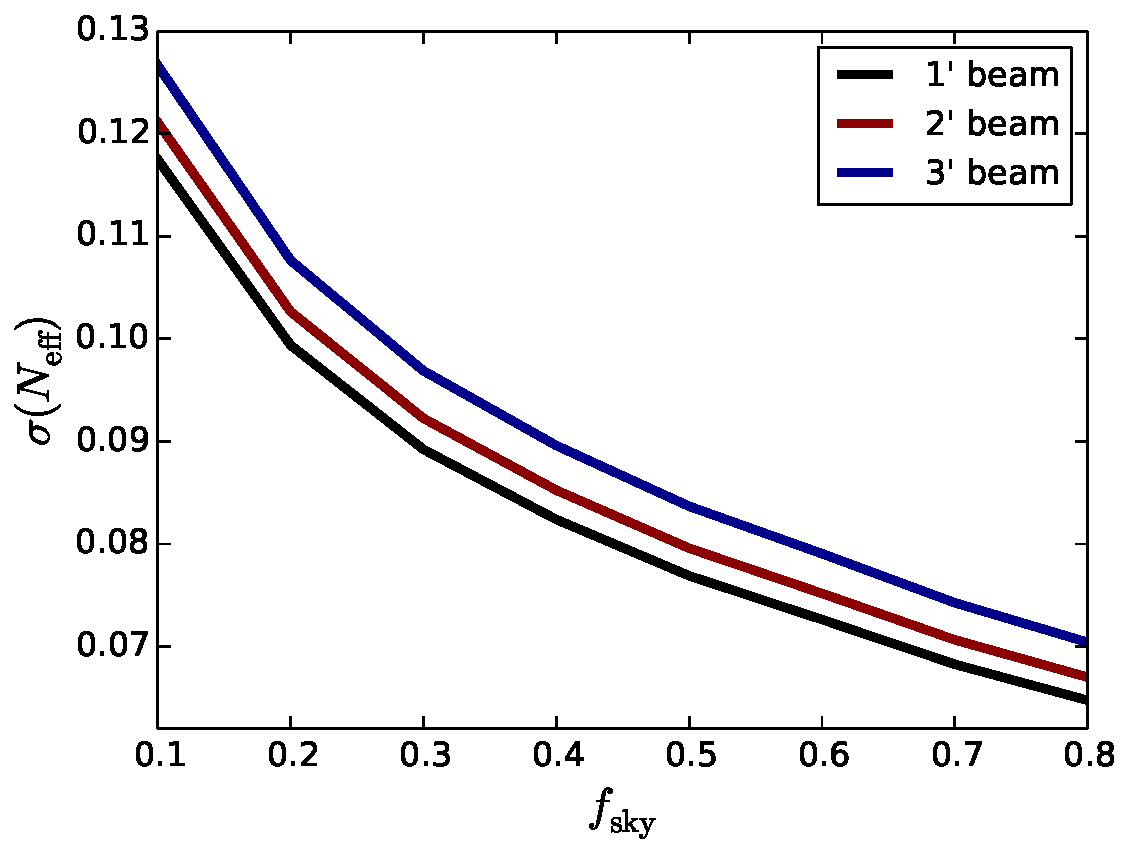
\includegraphics[width=0.48\textwidth]{Neutrinos/NfskyYp.pdf}
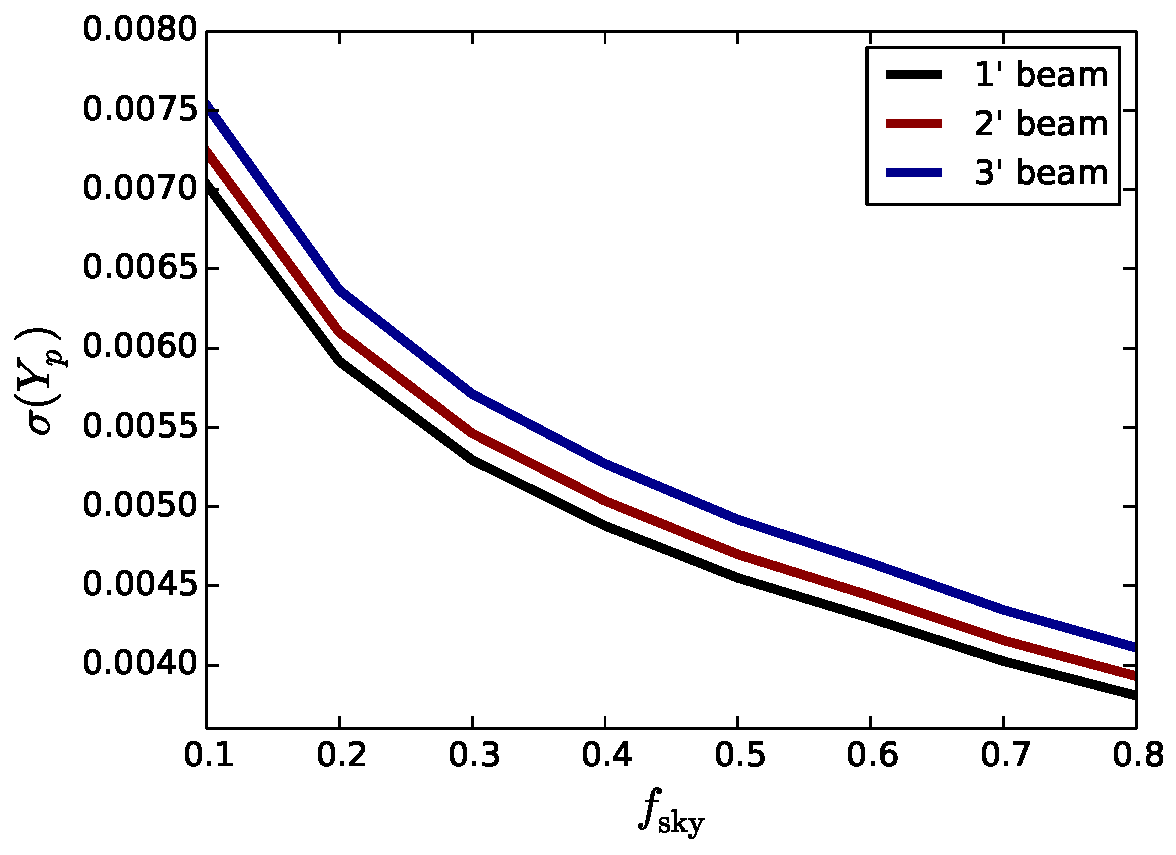
\includegraphics[width=0.5\textwidth]{Neutrinos/Ypfsky.pdf}
\caption{{\it Left:} Forecasts for $\sigma(\Neff)$, marginalized over $Y_p$, as a function of sky fraction for beam sizes of $1',2'$ and $3'$.  {\it Right :} Forecasts for $\sigma(Y_p)$, marginalized over $\Neff$, as a function of sky fractionfor beam sizes of $1',2'$ and $3'$.  For both figures, the sensitivity have been normalized to 1 $\mu$K-arcmin for $f_{\rm sky} =0.4$ and is scaled according to $S \propto f_{\rm sky}^{1/2}$ for different sky fractions.}
\label{fig:YpNeff_fsky}
\end{center}
\end{figure} 

Constraints on the combined $Y_p$-$\Neff$ parameter space is a useful probe of both the physics of BBN and recombination and possible evolution in between.  It is therefore useful to consider joint constraints on these two parameters available from the CMB alone.  

The leading effect of both $Y_p$ and $\Neff$ is to change the damping tail and they are therefore degenerate.  However, this degeneracy is broken both by the phase shift induced by neutrinos and by the $E$-mode spectra.  The phase shift is sensitive to delensing of the $T$ and $E$-modes and proper forecasting must account for realistic delensing, and the non-trivial covariance induced by the imperfect delensing.  Forecasts including both effects are given in Table~\ref{tab:YpNeffbeam}.

 

\begin{table}[t!]
\begin{center}
\begin{tabular}{l ccc} 
 \toprule
    		sensitivity / beamsize		    			& $1'$  		& $2'$  		& $3'$  		 \\ [0.5ex]
 \midrule
   1 $\mu$K-arcmin & 0.082 / 0.0049		& 0.085 /  0.0050 		& 0.090 / 0.0053		 		  \\
  2  $\mu$K-arcmin & 0.093 / 0.0054		& 0.096 / 0.0056		& 0.10 / 0.0058	 		  \\
   3  $\mu$K-arcmin & 0.10 / 0.0058		& 0.10 / 0.0059		& 0.11 / 0.0062		 		  \\
    \bottomrule
\end{tabular}
\caption{Forecasts for $\sigma(\Neff)$ / $\sigma(Y_p)$ with varying beamize in arcmin (') and detector sensitivity. These forecasts allow both $Y_p$ and $\Neff$ to vary (along with the parameters of $\Lambda$CDM).  We assume $f_{\rm sky} = 0.4$. }
\label{tab:YpNeffbeam}
\end{center}
\end{table}

Like the case of $\Neff$-only forecasts, constraints on $Y_p$ and $\Neff$ are primarily sensitive to $f_{\rm sky}$ as shown in Figure~\ref{fig:YpNeff_fsky}.  Although both parameters are sensitive to the damping tail and we also see the significant impact of varying the beamsize from $1'$ to $3'$.  




\section{Detection Scenarios for Labs and Cosmology}~\label{sec:neffscenarios}

Light particles are under active experimental searches in a number of different domains.  There are a number of possible situations where a discovery could be made in cosmology and/or the lab that could inform each other.

In this section, we will discuss plausible theoretical interpretations of a number of such scenarios.  Since there are numerous ways to produce a $\Delta\Neff$, these scenarios are not necessarily the only interpretations possible, but are nature interpretations within well studied theoretical frameworks.   

\subsection{Dark Sectors and Particle Physics}

Deviations from $\Neff = 3.046$ can arise from a wide variety of changes to the particle content and thermal history of the universe.  In most cases, the physics responsible fundamentally requires a coupling of new particles to the Standard Model in regimes where they often can, in principle, be detected by other means.  Cosmology is a very broad tool for searching for beyond the Standard Model physics, but it is also very complimentary to more targeted searches.  A list of plausible detection scenarios is shown in Table~\ref{table:darkscenarios}:
\begin{itemize}
\item Evidence for new massless particles from either experiments or astrophysical observations have immediate implications for cosmology.  Any non-cosmological probe of light particles necessarily requires a coupling of the field to the Standard Model.  A measurement suggesting the strength of the coupling for this particle implies an upper-limit on the freeze-out temperature.  One can then look for the contribution to $\Delta \Neff$ associated with the particle.  If no such contribution is detected, we could place an upper limit on the reheating temperature (or a lower limit for a detection).  Axions present the simplest such examples, as there are a number of experiments that could directly detect axion dark matter (such as ADMX and CASPEr).  A detection in either experiment would predict $\Delta\Neff \geq 0.027$ unless reheating was at sufficiently low temperatures.  The inferred bound in either experiment can be read off of Figures~\ref{fig:axionphoton} or~\ref{fig:axiondipole}.

\item A more complicated example is if a deviation for typical stellar cooling is observed, as has been suggested for white dwarfs.  In this case, there are a number of models that could produce the necessary additional cooling, but would predict $\Delta\Neff \geq 0.027$.  The precise value of $\Delta \Neff$ depends on the spin of the particle and nature of the coupling (which cannot be unambiguously inferred from cooling).  Evidence for additional dark radiation would provide strong support that there is anomalous cooling and would imply a spin for the new light particle through the observed $\Delta \Neff$ using Figure~\ref{fig:Neff_thermal}.

\item Any supersymmetric interpretation of a discovery at the LHC  would require the existence of a gravitino (in order to make gravity consistent with supersymmetry).  There are many such scenarios where there would be no direction indication of a gravitino and/or its mass from colliders.  In this context, a cosmological detection of $\Delta \Neff \sim 0.06$ would have a natural interpretation as a light gravitino but would place a strong upper limit on the absolute scale of supersymmetry breaking of roughly $10^5$ GeV.  

\item There are a variety of possibilities where we may observe $\Delta \Neff \gtrless 0$ which results from the decay of a massive particle after neutrino decoupling.  A change to $\Neff$ after BBN would imply that $\Neff$ as measured in the CMB could differ significantly from the value inferred from primordial abundances~\cite{Fischler:2010xz}.  From the CMB, we can measure $Y_p$ and $\Neff$ simultaneously which implies such a signature can even be internal to the CMB.  Similarly decays to photons after BBN can also produce $\mu$- or $y$-distortions to the CMB spectrum which could be correlated with $\Delta \Neff < 0$.
\end{itemize}


\begin{table}[t!]
\begin{center}
\begin{tabular}
{| l | c | p{5cm} | p{5cm} | }\hline Scenario & $\Delta \Neff$ & Experimental Input & Conclusion \\
\hline 
Axions & $\geq 0.027$  & Direct detection of axions & Lower-limit on the reheat temperature
\\[.2cm]
Low-reheating & $0$  & Direct detection of axions & Upper-limit on the reheat temperature
\\[.2cm]    
Stellar Cooling & $\geq 0.027$  & Anomalous Stellar cooling (e.g. white dwarfs) & Evidence for new light particle ; Spin determined by $\Delta \Neff$.  
\\[.2cm]    
Gravitinos & $\geq 0.057$  & LHC evidence for SUSY & Upper-limit on scale of SUSY breaking
\\[.2cm]  
Late Decays & $< 0$  & Spectral Distortions observed ($\mu$ or $y$) & Evidence for new massive particle; energy injection
\\[.2cm]
Evolving $\Neff$ & $> 0$  & Primordial abundances (BBN) consistent with $\Delta \Neff =0$ & Radiation density changed between BBN and Recombination
\\[.2cm]  
\hline 
\end{tabular}
\caption{Relation between particle physics experiments and cosmology.}
\label{table:darkscenarios}
\end{center}
\end{table} 

\subsection{Dark Sectors and Neutrino Mass}




\begin{figure}[t!]
\begin{center}
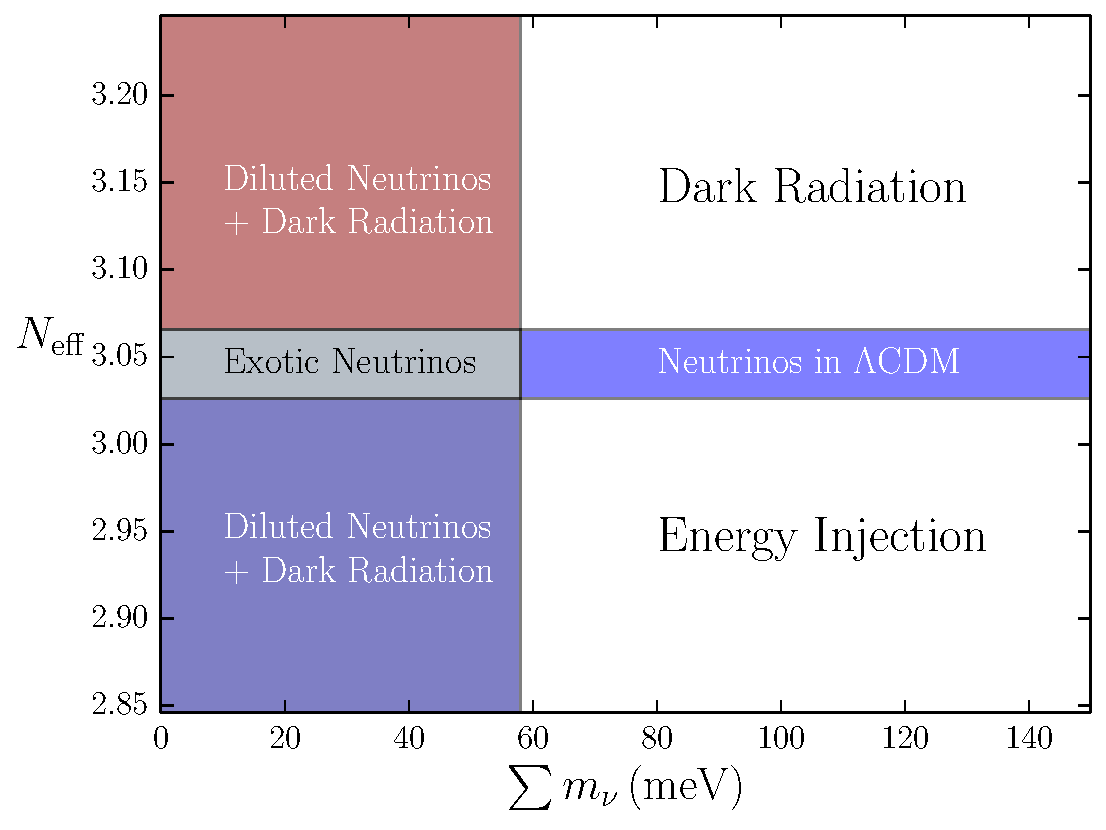
\includegraphics[width=0.65\textwidth]{Neutrinos/MnuNeff.pdf}
\caption{ Physical mechanisms behind different regions in the space $\Delta\Neff$ - $\sum m_\nu$.   }
\label{fig:MnuNeff}
\end{center}
\end{figure} 


CMB-S4 will provide compelling sensitivity in the $\Neff$-$\sum m_\nu$ plane.  From cosmology alone a measurement of $\sum m_\nu \gtrsim 60$ meV is consistent with conventional neutrino physics and therefore does not point to more exotic beyond the Standard Model physics without $\Neff$.  However, an upper limit or detection of $\sum m_\nu < 60$ meV would provide evidence of unconventional cosmology on its own and combined with $\Neff$ may give future insight into possible modifications to the cosmological history and/or neutrino physics necessary to accommodate such an observations.   An illustration of possible scenarios is shown in Figure~\ref{fig:MnuNeff} and can be compared directly to the forecasted region in Figure~\ref{fig:Neff_Mnu}:






\begin{itemize}


\item Conventional neutrino physics predicts $\sum m_\nu \gtrsim 60$ meV.  A measurement of $\Delta \Neff < 0.02$ (i.e. consistent with zero) is the expectation from $\Lambda$CDM.  As described in the previous subsection, $\Delta \Neff> 0$ suggests dark radiation or additional energy in neutrinos and $\Delta \Neff < 0$ would imply energy injection into photons after neutrino decoupling.  The amount of energy injection that is consistent with the current constraint from Planck, $\Neff = 3.04 \pm 0.18$, is insufficient to significantly alter $\sum m_\nu$, as it would correspond to at most a five percent change in $\Omega_\nu h^2$.



\begin{figure}[t!]
\begin{center}
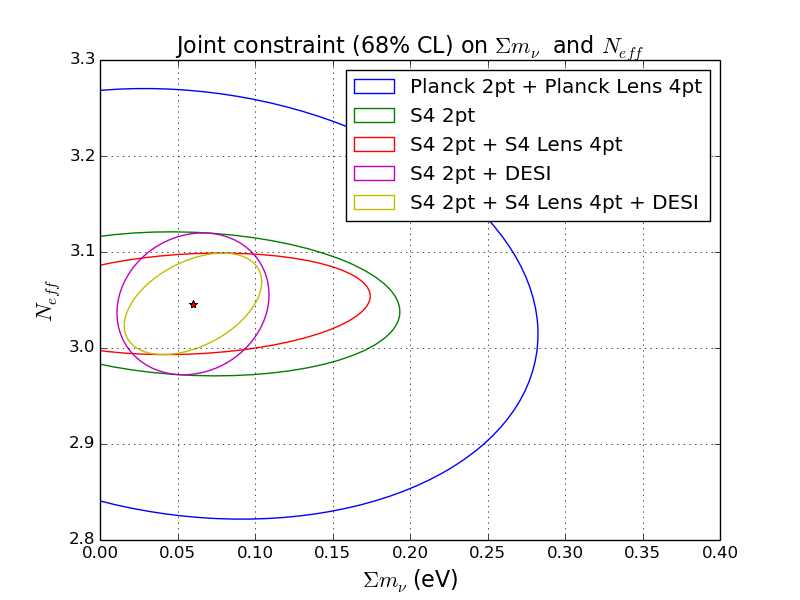
\includegraphics[width=0.65\textwidth]{Neutrinos/Neff_Mnu.png}
\caption{Forecasts 2d parameter space $\sigma(\Neff)$ and $\sigma(\sum m_\nu)$.  These constraints assume $f_{\rm sky} = 0.4$ and  1 $\mu$K-arcmin noise.  A prior of $\tau = 0.06 \pm 0.01$ was also assumed. }
\label{fig:Neff_Mnu}
\end{center}
\end{figure} 

\item If $\sum m_\nu < 60$ meV, the most natural explanation is that the number density of neutrinos was lowered due to a change to the standard cosmological evolution.  However, in order to significantly lower the number density to explain such an observation, the neutrinos number would have to be changed dramatically which, on its own, would be in contradiction with current $\Neff$ constraints.  Therefore, to satisfy existing constraints on $\Neff$ from Planck, some other form of radiation (i.e. other than Standard neutrinos) would also be required to make $|\Delta \Neff| < 0.2$.  Seeing a deviation of the form $\Delta \Neff \gtrless 0$ would give additional evidence for a modification of the thermal history.

\item If $\sum m_\nu < 60$ meV and $\Delta\Neff = 0$, then it suggests that either the mass for the neutrinos is generated after the CMB (late mass) or that the heavy neutrinos decayed to a lighter specifics in some novel way.  This situation would be unusual in that the limits on $\sum m_\nu$ would suggest deviations from the Standard thermal history without any other hints.  Presumably this scenario would be scrutinized heavily to check that the amplitude of the power spectrum is normalized correctly.  Finally, one might also allow for a delicate cancelation between the dilution of the neutrinos and the additional dark energy to be consistent with $\Delta \Neff =0$.




\end{itemize}





%%
%% Populate the .bib file with entries from SPIRES Bibtex (preferred)
%% or ADS Bibtex (if no SPIRES entry).
%%  SPIRES will also supply the CITATION line information; please include it.
%%


